% !TEX root = ../tls-cca-privacy.tex
\section{Verification of \\Metropolitan Area Network Traceability}\label{sec:verloc}
\label{sec:results}
This section emulates attacker (b) as defined in Section~\ref{sec:attacker}, which has interception capabilities in a \man.
We verify that this attacker can effectively track users through passive measurements.

\subsection{Experimental Setup and Methodology}\label{sec:exp}
To give a detailed analysis and evaluation of {\apns} communication patterns and
to be able to analyze the impact of {\apns}'s use of CCA on user privacy in the \man attacker scenario, we conduct an
extensive analysis of {\apns} communication. This scenario does not include
mobile cellular connections, but only WLAN and wired connections.


We monitor {\apns} communication at the Internet uplink of the Munich Scientific Network (MWN), a \man connecting about 100,000 users to the Internet.
We consider the MWN an insightful environment as it provides properties of scientific (connecting several large universities), corporate (employees at various organizations), and residential (student residence halls) networks.

Using \textit{tcpdump}, we capture {\apns} TLS handshake packets containing certificates over the course of 17 days.
We employ a \textit{pcap} filter for TCP traffic with destination ports 443, 5223, 2195, and 2196 used by {\apns} as described in Section~\ref{sec:apns}.
The filter also limits capturing to TLS handshake protocol
messages (\textit{Record Layer ContentType} = \textit{handshake}) containing certificate
information (\textit{Handshake Type} = \textit{Certificate}).

We capture data as \textit{pcap} files and use a python processing tool
leveraging \textit{scapy}~\cite{scapy} extended with
\textit{scapy-ssl\_tls}~\cite{scapytls} to extract certificate information.
Using this tool, we extract the following information from the \textit{pcap} files:

\begin{itemize}
	\item \textbf{Connections: }%
	timestamp, source IP address, source port, destination IP, destination port, certificates found
	\item \textbf{Certificates: }%
	X.509 version, serial number, subject, issuer, public key modulus, public key size, start and end of validity, fingerprint, extensions contained
	\item \textbf{Certificate extensions: }%
	name/OID and values
\end{itemize}

{\noindent}While processing, we perform DNS reverse resolution for source and destination IP addresses to obtain DNS hostnames.

\subsection{Ethical Considerations}\label{sec:ethical}

We follow an internal multi-party approval process before any measurement
activities are carried out. This approval process incorporates the proposal of
Partridge and Allman~\cite{partridge2016ethical} to assess whether the
collection of data can harm individuals and whether the collected data
reveals private information.

The focus of this work is solely to create profiles of devices. We do not
attempt create a link between devices (i.e., the certificates found) and the
respective owner's identity, except five members of our research group giving informed consent to case studies.
Information contained in the certificates does not provide a possibility to directly link it with a user. 
We neither try to link certificates to users based on identifiers such as IP addresses, nor try to uncover their geographical location.

The measurements conducted for this work were performed on an isolated measurement infrastructure not accessible from the Internet. 
Data obtained in our measurements must remain on this infrastructure. 
%
The methodology for this experiment was thoroughly documented before the measurement was conducted.
The experiment's methodology fully complies with the strict code of conduct required by our internal ethical review processes, and we obtained approval for our measurements in this process. 
We hence conclude it is ethical to conduct the experiment, but will, in contrast to our usual policy, not share raw data from this work with the public.


\subsection{Properties of {\apns} Certificates}
Our experiments show that \apns, relying on standard TLS 1.2, employs
standard X.509v3 certificates for mutual authentication between devices and
{\apns} servers. {\apns} devices use 1024 bit RSA keys and are provided with
certificates issued by an \textit{Apple iPhone Device CA} certificate authority
using the common name \texttt{\footnotesize{C=US, O=Apple Inc., OU=Apple iPhone,
CN=Apple iPhone Device CA}}.


Our investigations show that certificates of mobile devices (iPhones, iPads)
running iOS have different properties than certificates of desktop devices
running macOS and \itunes on Windows. This allows us to distinguish between mobile
and desktop devices: certificates for mobile devices have a subject containing a
unique identifier and CA information similar to
\texttt{\footnotesize{CN=7F3F3123\--1234\--4EF8\--5678\--F3CDE236E1EF, C=US,\-
ST\-=CA,\- L=Cupertino, O=Apple Inc., OU=iPhone}}. 
In contrast, certificates for desktop devices only contain the unique identifier:
\texttt{\footnotesize{CN=7F3F3123-1234\--4EF8\--5678\--F3C\-DE\-236\-E1EF}}.
By investigating several devices of consenting users, we verify that the certificate's \emph{``not valid before''} timestamp reflects the precise time of device registration with Apple.
The certificate validity for iOS devices is 3 years, while certificates for desktop devices only have a validity of 1 year.

\subsection{Data Capturing and Basic Statistics}
%
Capturing for 17 days in September 2016, we observe 70,173,492 TLS CCA connections with 57,477 unique client certificates, of which 56,128 (97\%) stem from \apns.
Across all 57,477 client certificates, we find 220 distinct issuer distinguished names (\textit{DNs}). % in those 57,477 client certificates, 
The Top 5 issuer \textit{DNs} are shown in Table~\ref{tab:issuercn}, exhibiting a clear dominance of {\apns} certificates in our data set, 
but also showing other use cases of CCA such as client service authentication and remote device management.

\begin{table}
	\centering
	\caption{Number of observed TLS client certificates for five most frequent Issuer Distinguished Names.}%
	 \resizebox{\columnwidth}{!}{
	\begin{tabular}{ll}
		\toprule
		\#Certs & Issuer Distinguished Name \\
		\midrule
		56128 & /C=US/O=Apple Inc./OU=Apple iPhone/CN=Apple iPhone Device CA \\
		334 & /CN=Layer Client CA/C=US/L=San Francisco/O=Layer, Inc/ST=CA \\
		221 & /CN=AnyDesk Client \\
		76 & /C=KR/ST=Kyunggido/L=Suwon/O=Samsung Electronics (\textit{redacted})\\ 
		52 & /CN=Ricoh Remote Service (\textit{redacted})\\ 
		\bottomrule
	\end{tabular}
	}
	\label{tab:issuercn}
	\vspace{-1em}
\end{table}

The 56,128 {\apns} certificates can further be broken down into 40,313 (72\%) iOS certificates and 15,815 (28\%) desktop certificates.
Of the 70,173,492 TLS CCA connections, we identify 68,231,915 as {\apns} certificates on port 5223 and 1,588,864 as {\apns} certificates on port 443.
The small remainder of 352,713 connections did not use {\apns} certificates.

\subsection{Recurrence of Certificates}
To assess whether the described capture would allow for reliable traceability of users, we first investigate the recurrence of certificates: Only certificates observed more  than once allow for a basic level of user tracking. Figure~\ref{fig:connspercert} displays the number of connections observed per certificate.

\begin{figure}%
	\centering
	\begin{subfigure}{\columnwidth}%{0.48\textwidth}%
		\href{https://github.com/tumi8/cca-privacy/blob/master/analyses/results/1_connections_per_certificate.ipynb}{%
		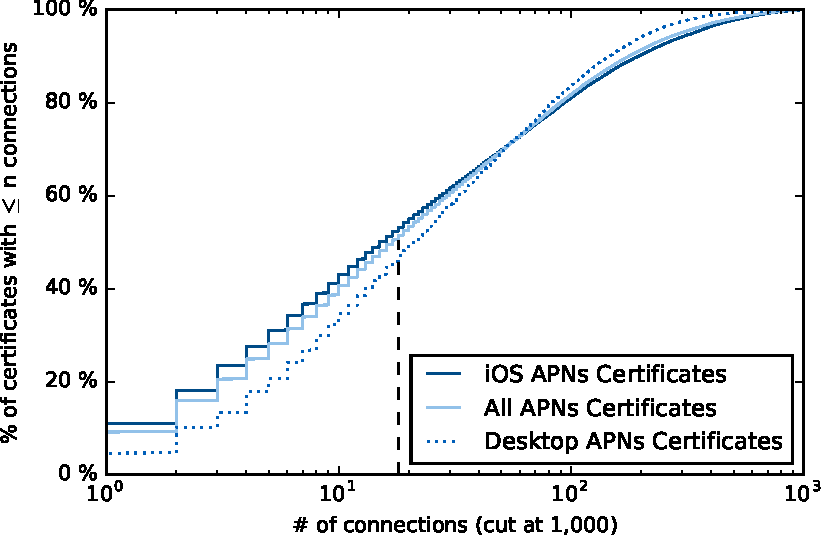
\includegraphics[width=\textwidth]{figures/connspercert-crop.pdf}%
		}
		\caption{$\sim$50\% of certificates observed with more than 17 connections, 9\% of certificates only observed once (5\% desktop, 11\% iOS).}
		\label{fig:connspercert}
	\vspace{3mm} % manually align figure layout
	\end{subfigure}
	\begin{subfigure}{\columnwidth}%{0.48\textwidth}%
		\href{https://github.com/tumi8/cca-privacy/blob/master/analyses/results/1_connections_per_certificate_per_day.ipynb}{%
		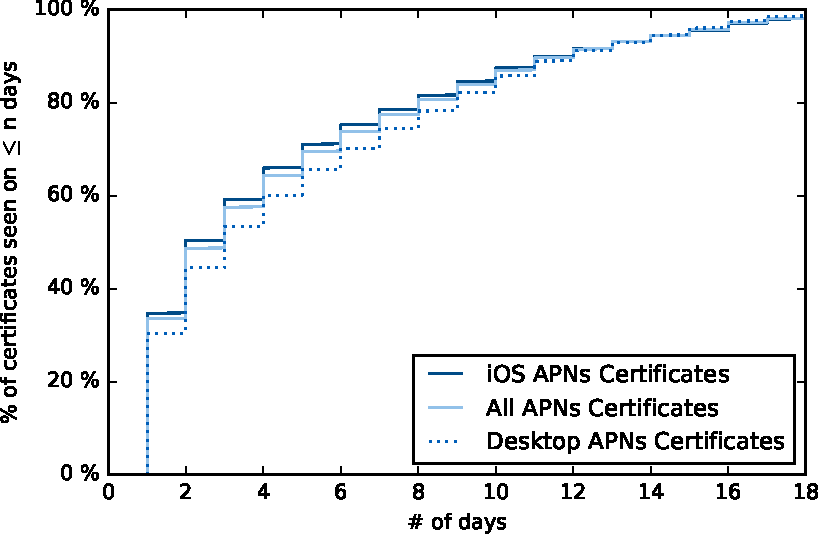
\includegraphics[width=\textwidth]{figures/connspercert_per_day-crop.pdf}%
		}
		\caption{50\% of certificates observed on 3 or more separate days, 34\% only observed on 1 day (30\% desktop, 35\% iOS).}
		\label{fig:connspercert_per_day}
	\end{subfigure}
	\caption{Statistics on certificate recurrence --- \emph{Click on any data-driven figure in this paper to go to its source code}}
	\label{fig:connspercert_big}
	\vspace{-3mm} % avoid ugly linebreak in section V-F
\end{figure}

We display total number as well as a breakdown into iOS and desktop devices. We
find about 50\% of total certificates to have 17 or more connections. The fact
that only $\leq$10\% of certificates are only observed once speaks to
traceability of individual certificates. Please note that 95\% of desktop
certificates were observed more than once, as desktop devices typically can not connect
to {\apns} through cellular service, hence always use our observed WLAN or wired connections to
connect. We find some certificates with dozens of millions of connections, which
we can link to an iOS continuous integration build cluster within the network.
Figure~\ref{fig:connspercert_per_day} displays the number of days that
individual certificates were observed to connect on. About 50\% of certificates
connected on 3 or more days. We consider these regular users of our network,
which are likely well traceable over longer periods.

\subsection{Deductions about User Behavior}
We next set out to explore the level of insight that can be deduced about
individual users and devices.

Figure~\ref{fig:userstudy-1} tracks the {\apns} certificate of one of
the authors' MacBook to ensure applicability of our methodology and
highlight the relevance of our work. Based on the subnet of the source IP address, we can
track whether this user logged in from his desk, through WLAN, or through VPN.
% 
Days off and days with outside meetings can clearly be identified, for example, 
the first Monday, with a remote VPN login followed by desk presence later that day.
Meetings away from desk are visible through WLAN logins, for example, the second
Wednesday and Thursday. 
This exhibits the power of tracking users from \apns certificates at a \man level. 
This information is also accessible to eavesdroppers on the path between this \man and the {\apns} backend. 
The mapping of IP addresses to certain networks and characteristics may seem difficult for outsiders, but is eased by descriptive reverse DNS names deployed in these networks.

\begin{figure}%
	\centering
		\href{https://github.com/tumi8/cca-privacy/blob/master/userstudy/userstudy.ipynb}{%
		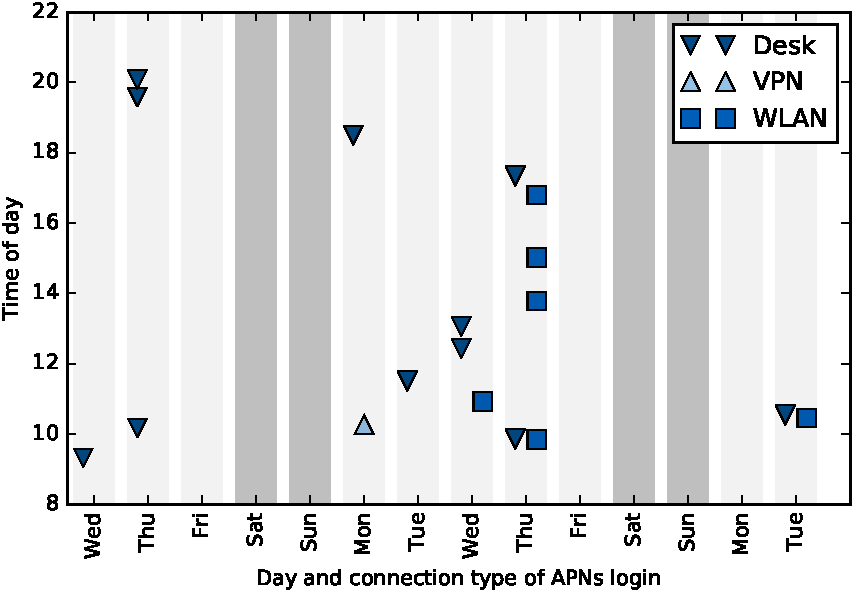
\includegraphics[width=.94\columnwidth]{figures/userstudy-crop.pdf}%
		}
		\caption{User Study: {\apns} logins clearly show work starting times and locations (derived from subnet data).}
		\label{fig:userstudy-1}
		\vspace{-3mm}
\end{figure}
\subsection{Deductions about Devices}

As the certificate's \emph{``not valid before''} timestamp reflects the precise time of device registration with Apple, this can narrow down the device type, as Apple typically stops selling
previous hardware models with the availability of new devices. This means that
the majority of certificates created at a certain point of time will belong to devices from the Apple hardware offerings at that time.

Figure~\ref{fig:certsvalid} depicts the cumulative distribution of the ``\emph{not valid before}'' timestamps in observed {\apns} certificates.
%
\begin{figure}%
	\href{https://github.com/tumi8/cca-privacy/blob/master/analyses/results/2_certificates_valid_from_anon.ipynb}{%
	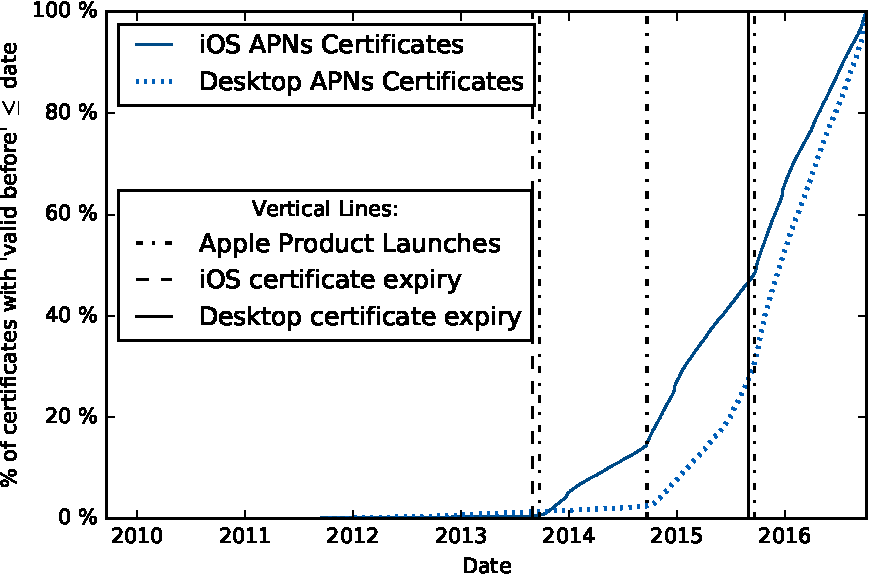
\includegraphics[width=\columnwidth]{figures/certs_valid_from-crop.pdf}%
	}
	\caption{CDF of ``\emph{not valid before}'' timestamps of {\apns} certificates. Highlighted are the influence of Apple's end of September product launches as well as the expiry threshold dates for iOS certificates, which are valid for three years, and desktop certificates, which are valid for one year.}
	\label{fig:certsvalid}
\end{figure}%
Several observations can be taken from this figure:

First, certificates are used beyond their expiry date. As certificates are
valid for 3 years for iOS and 1 year for desktop devices, we can plot the expiration threshold
of certificates in Figure~\ref{fig:certsvalid}.
Certificates issued before these thresholds have exceeded their validity period.

We can see that 28\% of desktop and 1\% of mobile devices use expired certificates.
% source for 28% and 1% numbers:  jupyter notebook analyses/results/2_certificates_valid_from.ipynb
We conclude that {\apns} clients do not systematically renew their certificates and only
re-installations or re-registrations cause certificate renewals over time.
This lack of systematical certificate renewal extends the possible duration a device
can be traced.
Furthermore, Apple's product presentations in end of September typically boost registration of new devices and therefore certificates.
